
\chapter{Operads}

The Operad structure generalises the idea of composition for operators which input \( n \) objects and output \( 1 \). 
Operators of this form are given the name \( n \)-ary operators and we compose \( n \)-ary operators using the composition operation \( \circ_i \) which composes the second operator into the \( i \)th input to the first operator.

\section{Examples of Operads}  \label{sec:examples}

\begin{Example}[Operad of real multi-linear functions]
We will define
\[ \mathit{M}(n) = \{ f \mid f \map{\R^n}{\R} \text{ where \( f \) is a real multi-linear function} \} \]
as the set of \( n \)-ary multi-linear functions in the real numbers.
As an example we designate \( A \in \mathit{M}(3) \) and \( B \in \mathit{M}(2) \) and express the composition of \( B \) into the second argument of \( A \) as.
\[ A \circ_2 B (x_1, x_2, x_3, x_4) = A(x_1, B(x_2, x_3), x_4) \]
With an intuitive notion of composition of functions. 
It's of note that \( A \circ_2 B \in \mathit{M}(3 + 2 - 1) \) because the \( 2 \) inputs of \( B \) replaced one of the \( 3 \) inputs of \( A \). 
\end{Example}

\begin{Example}[Little \( 2 \)-cubes Operad] \label{ex:squares}
    
Let's first define a solid square with side length \( l \in \R \) and centre \( \omega \in \C \) by
\[ S_{\omega, l} = \set{ z \in \C \mid |Re(z) - \omega| \leq l / 2 \text{ and } |Im(z) - \omega| \leq l / 2 } \]
The \( n \)-squares Operad \( \{ S(n) \}_{n \ge 1} \) is described by~\cite{spivak2013categorytheoryscientistsold}~as disjoint squares in \( S_{0, 1} \), where \( S(n) \) represents the configuration of \( n \) disjoint squares in \( S_{0, 1} \) and composition of square configurations is defined by replacing squares with configurations. 
For example, we might describe \( A \in S(3) \) and \( B \in S(2) \) by the following diagrams. 
\begin{center}
    \begin{tikzpicture}
        \node[left] at (-1.5, 0) {\( A = \)};
        \Square at (0, 0) length (1.5) {}; % Main square
        \Square at (-0.8, 0.6) length (0.5) {\( 1 \)};
        \Square at (0.5, 0.7) length (0.75) {\( 2 \)};
        \Square at (0.2, -0.8) length (0.6) {\( 3 \)};
    \end{tikzpicture} \hspace{1cm}
    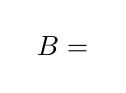
\begin{tikzpicture}
        \node[left] at (-1.5, 0) {\( B = \)};
        \Square at (0, 0) length (1.5) {};
        \Square at (-0.6, -0.6) length (0.5) {\( 1 \)};
        \Square at (0.4, 0.7) length (0.7) {\( 2 \)};
    \end{tikzpicture} 
    \hfill
\end{center} 
If we do so then we can define composition \( A \circ_{i} B \) as replacing square \( A_i \) with configuration \( B \). 
For example the composition of \( B \) into \( 2 \) is the following, where the dotted line represents the outline of where \( 2 \) was. 
\begin{center}
    \begin{tikzpicture}
        \node[left] at (-1.5, 0) {\( A \circ_{2} B= \)};
        \Square at (0, 0) length (1.5) {}; 
        \Square at (-0.8, 0.6) length (0.5) {\( 1 \)};
        % \Square at (0.5, 0.7) length (0.75) {};
        \draw[densely dashed] (-0.25, -0.05) rectangle (1.25, 1.45);
        \Square at (0.5 - 0.3, 0.7 - 0.3) length (0.25) {\( 1' \)};
        \Square at (0.5 + 0.2, 0.7 + 0.35) length (0.35) {\( 2' \)};
        \Square at (0.2, -0.8) length (0.6) {\( 3 \)};
    \end{tikzpicture} \hfill \\
\end{center}

\begin{Exercise}
    Determine the precise formula for the composition described above in terms of the location and side lengths of the original configurations of squares. 
\end{Exercise}
\end{Example}

% \begin{Example}[Operad of Parenthesised Permutations]
% The operad of parenthesised permutations \( \mathit{Pa} \) (by~\cite{merkulov2021grothendieckteichmuellergroupoperadsgraph}) is an operad where for a given finite set of elements \( I \), we define \( \mathit{Pa}(I) \) as the set of parenthesised permutations of the elements of \( I \).

% For example, \( (2(3(14))) \in \mathit{Pa}(\{ 1, 2, 3, 4 \}) \) and \( (a(cb)) \in \mathit{Pa}(\{ a, b, c \}) \).
% Let's consider the composition of these elements:
% \[ (2(3(14))) \circ_2 (a(cb)) = ((a(cb))(3(14))) \in \mathit{Pa}([4] \setminus \{ 2 \} \sqcup \{ a, b, c \}) \]

% Note that as opposed to the other examples where \( \circ_2 \) represented replacing the second spot of the input, \( \circ_2 \) in this example represents replacing the value \( 2 \) in \( (2(3(14))) \). 
% You will also note that in the first example we had a number \( n \) as input to \( M \), whereas here we're considering finite sets as inputs to \( Pa \). 
% This distinction is explained in \cref{sec:specialisation}.

% \begin{Exercise}
%     For a given finite set \( I \) count the number of elements in \( Pa(I) \) and for another finite set \( J \) and \( i \in I \), count the number of elements in \( Pa(I) \circ_i Pa(J) \). 
% \end{Exercise}

% \end{Example}

\section{Definition of an Operad}
There exist many definitions of an Operad which equivalently define the same structure, which generally includes the following data. 
\begin{enumerate}
    \item A sequence of collections of operators \( \{ \Op(n) \}_{n \ge 0} \) of various arity.
    \item Permutations maps for the inputs to each operator. 
    \item A composition operation \( \circ_i \map{\Op(n) \times \Op(m)}{\Op(n + m - 1)}\) between these operators.
    \item A unit, \( e \in \Op(1) \), a \( 1 \)-ary function which acts as an identity.  
\end{enumerate}

\begin{Remark}
We will consider a specialisation of the definition of the operad by \cite{merkulov2021grothendieckteichmuellergroupoperadsgraph} which acts similarly to the definition by \cite{spivak2013categorytheoryscientistsold}. 
\end{Remark}


% The following definition~(from \cite{merkulov2021grothendieckteichmuellergroupoperadsgraph}) will give a general definition of a operad in a symmetric monoidal category \( C \) within the groupoid of finite sets, \( S \).
% We will then consider a specialisation of our definition in  \cref{sec:specialisation}, given by~\cite{spivak2013categorytheoryscientistsold}~and many other sources, which is easier to reason about. 

% \begin{Remark}
% A symmetric monoidal category \( C \) is simply a category with a product \( \otimes \) and associative \( \Phi \) and commutative \( \beta \) maps with a unit \( \mathbb{1}_C \) with isomorphisms \( \lambda \) and \( \rho\) as left and right simplification maps.
% A groupoid is a category in which all morphisms are endomorphisms and so the groupoid of finite sets contains all finite sets as objects, and all permutations of finite objects as morphisms.
% \end{Remark}

\subsection{Objects and Permutations}
% An Operad \( \Op \) over \( C \) consists of an \( S \)-module, which is a functor \( \Op: S \rightarrow C \). 
% An \( S \)-module encodes the idea of permutations into the operad structure, since a permutation within \( S \) maps directly to a morphism in \( C \). 
% The objects of the Operad are the objects of the category, \( C \).
An Operad \( \Op \) over a category \( C \) is a functor from the permutation category \( \Sn \) to the category \( C \). 
\( \Sn \) contains natural numbers as objects and morphisms as permutations, i.e. \( \Ob(\Sn) := \N \) and \( \Hom_\Sn(n, m) := \Sn_n \) if \( n = m \), \( \emptyset \) otherwise. 

The morphisms of \( C \) are the image of the permutations in \( \Sn \) and so \( C \) has a natural concept of permutation, i.e. for a given permutation in \( \Sn \) which permutes \( [n] \), this maps to a morphism in \( C \) which permutes the inputs of the operators by that permutation. 

\subsection{Composition}
We define composition for two arities \( n, m \in \N \) as a bifunctor
\[ \circ_i \map{\Op(n) \times \Op(n)}{\Op(n + m - 1)} \]
Where associativity rules hold, i.e. for \( n, m, k \in \N \), indices \( i_1, i_2 \in [n] \) where \( i_1 \neq i_2 \), and operators \( A \in \Op(n), B \in \Op(m), \) and \( C \in \Op(k) \)
\[ (A \circ_{i_1} B) \circ_{i_2} C = (A \circ_{i_2} C) \circ_{i_1} A \]
And for indices \( i \in [n] \) and \( j \in [m] \)
\[ (A \circ_i B) \circ_j C = A \circ_i (B \circ_j C) \]
Where indices of the inputs to the operators aren't changed after composition, similarly to \cref{ex:squares}.

\subsection{Unit}
The unit \( e \in \Op(1) \) is a \( 1 \)-ary function which for a given arity \( n \in \N\), for any \( i \in [n] \) and operator \( f \in \Op(n) \) we know
\[ f =  f \circ_i e = e \circ_1 f \]

\subsection{The components of an Operad}
We now have a sequence of collections of operators \( \{ \Op(n) \}_{n \ge 0} \) such that \( \Op(n) \) is the \( n \)-ary operators in \( C \), a composition operation \( \circ_i \map{\Op(n) \times \Op(m)}{\Op(n + m - 1)} \), the morphisms of \( C \) as images of permutations is our interactions with permutations, and our unit \( e \) has been defined appropriately to admit the natural notions of the identity.

% We therefore consider composition and the properties it imposes. 
% Composition \( \circ_i^{I, J} \) for finite sets \( I, J \) and \( i \in I \), is a bifunctor.
% \[ \circ_i^{I, J}:  \Op(I) \otimes_C \Op(J) \rightarrow \Op(I \setminus \{ i \} \sqcup J ) \]

% The composition operation requires the following conditions which encodes associativity of the composition operation. 
% Consider finite sets \( I, J, K \) and let \( i, i_1, i_2 \in I \) and \( j \in J \) such that \( i \neq j \), then the following diagrams commute. 

% \[
%     \begin{tikzcd}[column sep=0.1cm]
%         & \Op(I \setminus \{ i_1\} \sqcup K) \otimes_C \Op(K) \ar[dr, "\circ_{i_2}^{I \setminus \{ i_1 \} \sqcup J, K}"] 
%         & \\
%     \Op(I) \otimes_C \Op(J) \otimes_C \Op(K) \ar[ur, "\circ_{i_1}^{I, J} \otimes \Id"] \ar[d, "id \otimes \beta"]
%         & 
%         & \Op(I \setminus \{ i_1, i_2 \} \sqcup J \sqcup K) \ar[d, equal] \\
%     \Op(I) \otimes_C \Op(K) \otimes_C \Op(J) \ar[dr, "\circ_{i_2}^{I, K} \otimes \Id"]
%         & 
%         & \Op(I \setminus \{ i_1, i_2 \} \sqcup K \sqcup J) \\
%         & \Op(I \setminus \{ i_2 \} \sqcup K) \otimes_C \Op(J) \ar[ur, "\circ_{i_1}^{I \setminus \{ i_2 \} \sqcup K, J}"] & \\
%     \end{tikzcd}
% \]
% \[
%     \begin{tikzcd}[column sep=tiny]
%         & \Op(I \setminus \{ i\} \sqcup J) \otimes_C \Op(K) \ar[dr, "\circ_j^{I \setminus \{ i \} \sqcup J, K}"] & \\
%     \Op(I) \otimes_C \Op(J) \otimes_C \Op(K) \ar[ur, "\circ_i^{I, J} \otimes \Id"] \ar[dr, "\Id \otimes \circ_j^{J, K}"]
%         &
%         & \Op(I \setminus \{ i \} \sqcup J \setminus \{ j \} \sqcup K) \\
%         & \Op(I) \otimes \Op(J \setminus \{ j \} \sqcup K) \ar[ur, "\circ_j^{I,J \setminus \{ j \} \sqcup K}"] & \\
%     \end{tikzcd}
% \]

% \subsection{Unit}
% We will also introduce a unit morphism \( e : \mathbb{1}_C \rightarrow \Op(A) \) for any one element set \( A \) with \( \bullet \in A \). 
% In which case the follow describes the identity map. 
% \[
% \begin{tikzcd}
%     \Op(I) \ar["\rho_{\Op(I)}^{-1}"]{r} & \Op(I) \otimes \mathbb{1}_C \ar["\Id \otimes e"]{r} & \Op(I) \otimes \Op(A) \ar["\circ_i^{I, A}"]{r} & \Op(I)
% \end{tikzcd}
% \]
% \[
% \begin{tikzcd}
%     \Op(I) \ar["\lambda_{\Op(I)}^{-1}"]{r} & \mathbb{1}_C \otimes \Op(I) \ar["e \otimes \Id"]{r} & \Op(A) \otimes \Op(I) \ar["\circ_\bullet^{A, I}"]{r} & \Op(I)
% \end{tikzcd}
% \]


% \section{Specialisation of Operads} \label{sec:specialisation}

% Our definition of an Operad is extremely general and encompasses any operad structure, however we use a slightly weaker definition from~\cite{spivak2013categorytheoryscientistsold}.
% We consider the permutation category, \( \Sn \) instead of the groupoid of finite sets, \( S \), and so each element is of the form \( [n] \) for \( n \in \N \) and morphisms are permutations.
% We can then consider an \( \Sn \)-module by \( \Op : \Sn \to C \). 

% We identify \( [n] \setminus \{ i \} \sqcup [m] \) with the set.
% \[ \{ 1, 2, 3, \cdots, i - 1, \underbrace{1^\prime,  2^\prime, 3^\prime, \cdots, (m - 1)^\prime}_{\text{Replacing the \( i \)th spot}},  i + 1, \cdots n - 1, n \} \]
% and the set \( [m + n - 1] \). 
% And therefore we define \( \Op(n) := \Op([n]) \) and thus we can equivalently characterise our \( \mathbb{S} \)-module as a sequence \( \{ \Op(n) \}_{n \in \N_{\ge 0}}\). 

% I will be inputting numbers and sets into \( \Op \) interchangeably and when the sets are evident we will write \( \circ_i \) instead of \( \circ_i^{I, J} \).
% This also implies that \( \Op(n + m - 1) := \Op([n] \setminus \{ i \} \sqcup [m]) \), and thus our composition operation can be rewritten nicely as.
% \[ \circ_i : \Op(n) \otimes \Op(m) \rightarrow \Op(n + m - 1) \]

% We now have a sequence of structures \( \{ \Op(n) \}_{n \in \N_{\ge 0}} \) containing objects from the category \( C \), a composition operation \( \circ_i \), our interaction with permutations comes from the definition of our \( \Sn \)-module mapping from \( \Sn \), and our unit morphism has been defined appropriately to admit the natural notions of the identity. 

% \begin{Exercise}
%     Consider notation used in examples from \cref{sec:examples} determine whether they're using the definition of the Operad or it's specialisation. 
    
%     Specifically consider the notation used for the \( \circ_a \) operator, whether \( a \) is an index for the input or an element of the Operad. 
% \end{Exercise}
\begin{Exercise}
    Show that our examples from \cref{sec:examples} are Operads.
\end{Exercise}
